\documentclass[conference]{IEEEtran}
\usepackage[utf8]{inputenc}
\usepackage{graphicx}
\usepackage{amsmath, amssymb}
\usepackage{caption}
\usepackage{subcaption}
\usepackage{hyperref}
\usepackage{booktabs}
\usepackage{float}      % for [H] float placement
\usepackage{placeins}
\usepackage{cite}
\hypersetup{
    colorlinks=true,
    linkcolor=blue,
    urlcolor=blue,
    }

\title{Predicting Prices for Used Cars}
\author{
    \IEEEauthorblockN{Julios Fotiou}
    \IEEEauthorblockN{Andreas Hadjoullis}
    \IEEEauthorblockA{
        Computer Science \\
        University of Cyprus \\
    }
}

\begin{document}

\maketitle

\section{Goals}
The automotive market has a wide range of car prices depending on factors such
as brand, age, mileage, and vehicle type. Predicting car prices accurately is
valuable for both buyers and sellers. This project aims to build a predictive
model using structured automotive data.

Our dataset is derived from
\href{https://www.kaggle.com/datasets/thedevastator/uncovering-factors-that-affect-used-car-prices/data}{Kaggle}
in which we have a comprehensive collection of valuable data about used cars,
and provides insight into how the cars are being sold, what price they are
being sold for, and all the details about their condition.

This project focuses on predicting car prices using machine learning models
trained on our real-world dataset. To improve prediction quality, extreme
values outside the practical range [1,000 – 200,000] are excluded. Various
regression models are evaluated using standardized preprocessing and feature
selection pipelines. We have also tested various classification algorithms on
our dataset, after splitting our dataset into bins, decided by their price.

The main goals of the project are:
\begin{itemize}
    \item Understand our dataset.
    \item Clean and preprocess raw car listing data.
    \item Select relevant features and remove noise.
    \item Train and compare multiple regression and classification models.
    \item Evaluate model performance using robust statistical metrics.
\end{itemize}

\section{Approach}
\subsection{Exploratory Data Analysis (EDA)}
First of all we need to understand our dataset. Before doing that however, we
get rid of all rows/instances in which the price does not belong in the range
of [1,000 – 200,000]. Our rezoning behind this choice, is that we only find our
model practical for values that lie in said range, and all other rows would
make it harder for the models to predict accurately prices in our desired
target range. After removing said rows, we end up with 288,023 rows instead of
the original 371,528.

We start by checking for features that have little to no deviation. For example
'offerType' only has two unique values, and one of them appears four times.
Meaning this feature has no impact on the target of our dataset. The same
applies for 'seller' and 'nrOfPictures'. So we remove the aforementioned
features after also removing the insignificantly few rows that had a different
value. We are now only working with 17 features/columns.

Some features, such as, 'vehicleType', 'gearbox', 'model', 'fuelType' and
'notRepairedDamage', have a significant number of missing values into the tens
of thousands.

\subsubsection{Target Variable - Price}
We start examining our target variable. This is the distribution of Car Prices:

\begin{figure}[H]
\centering
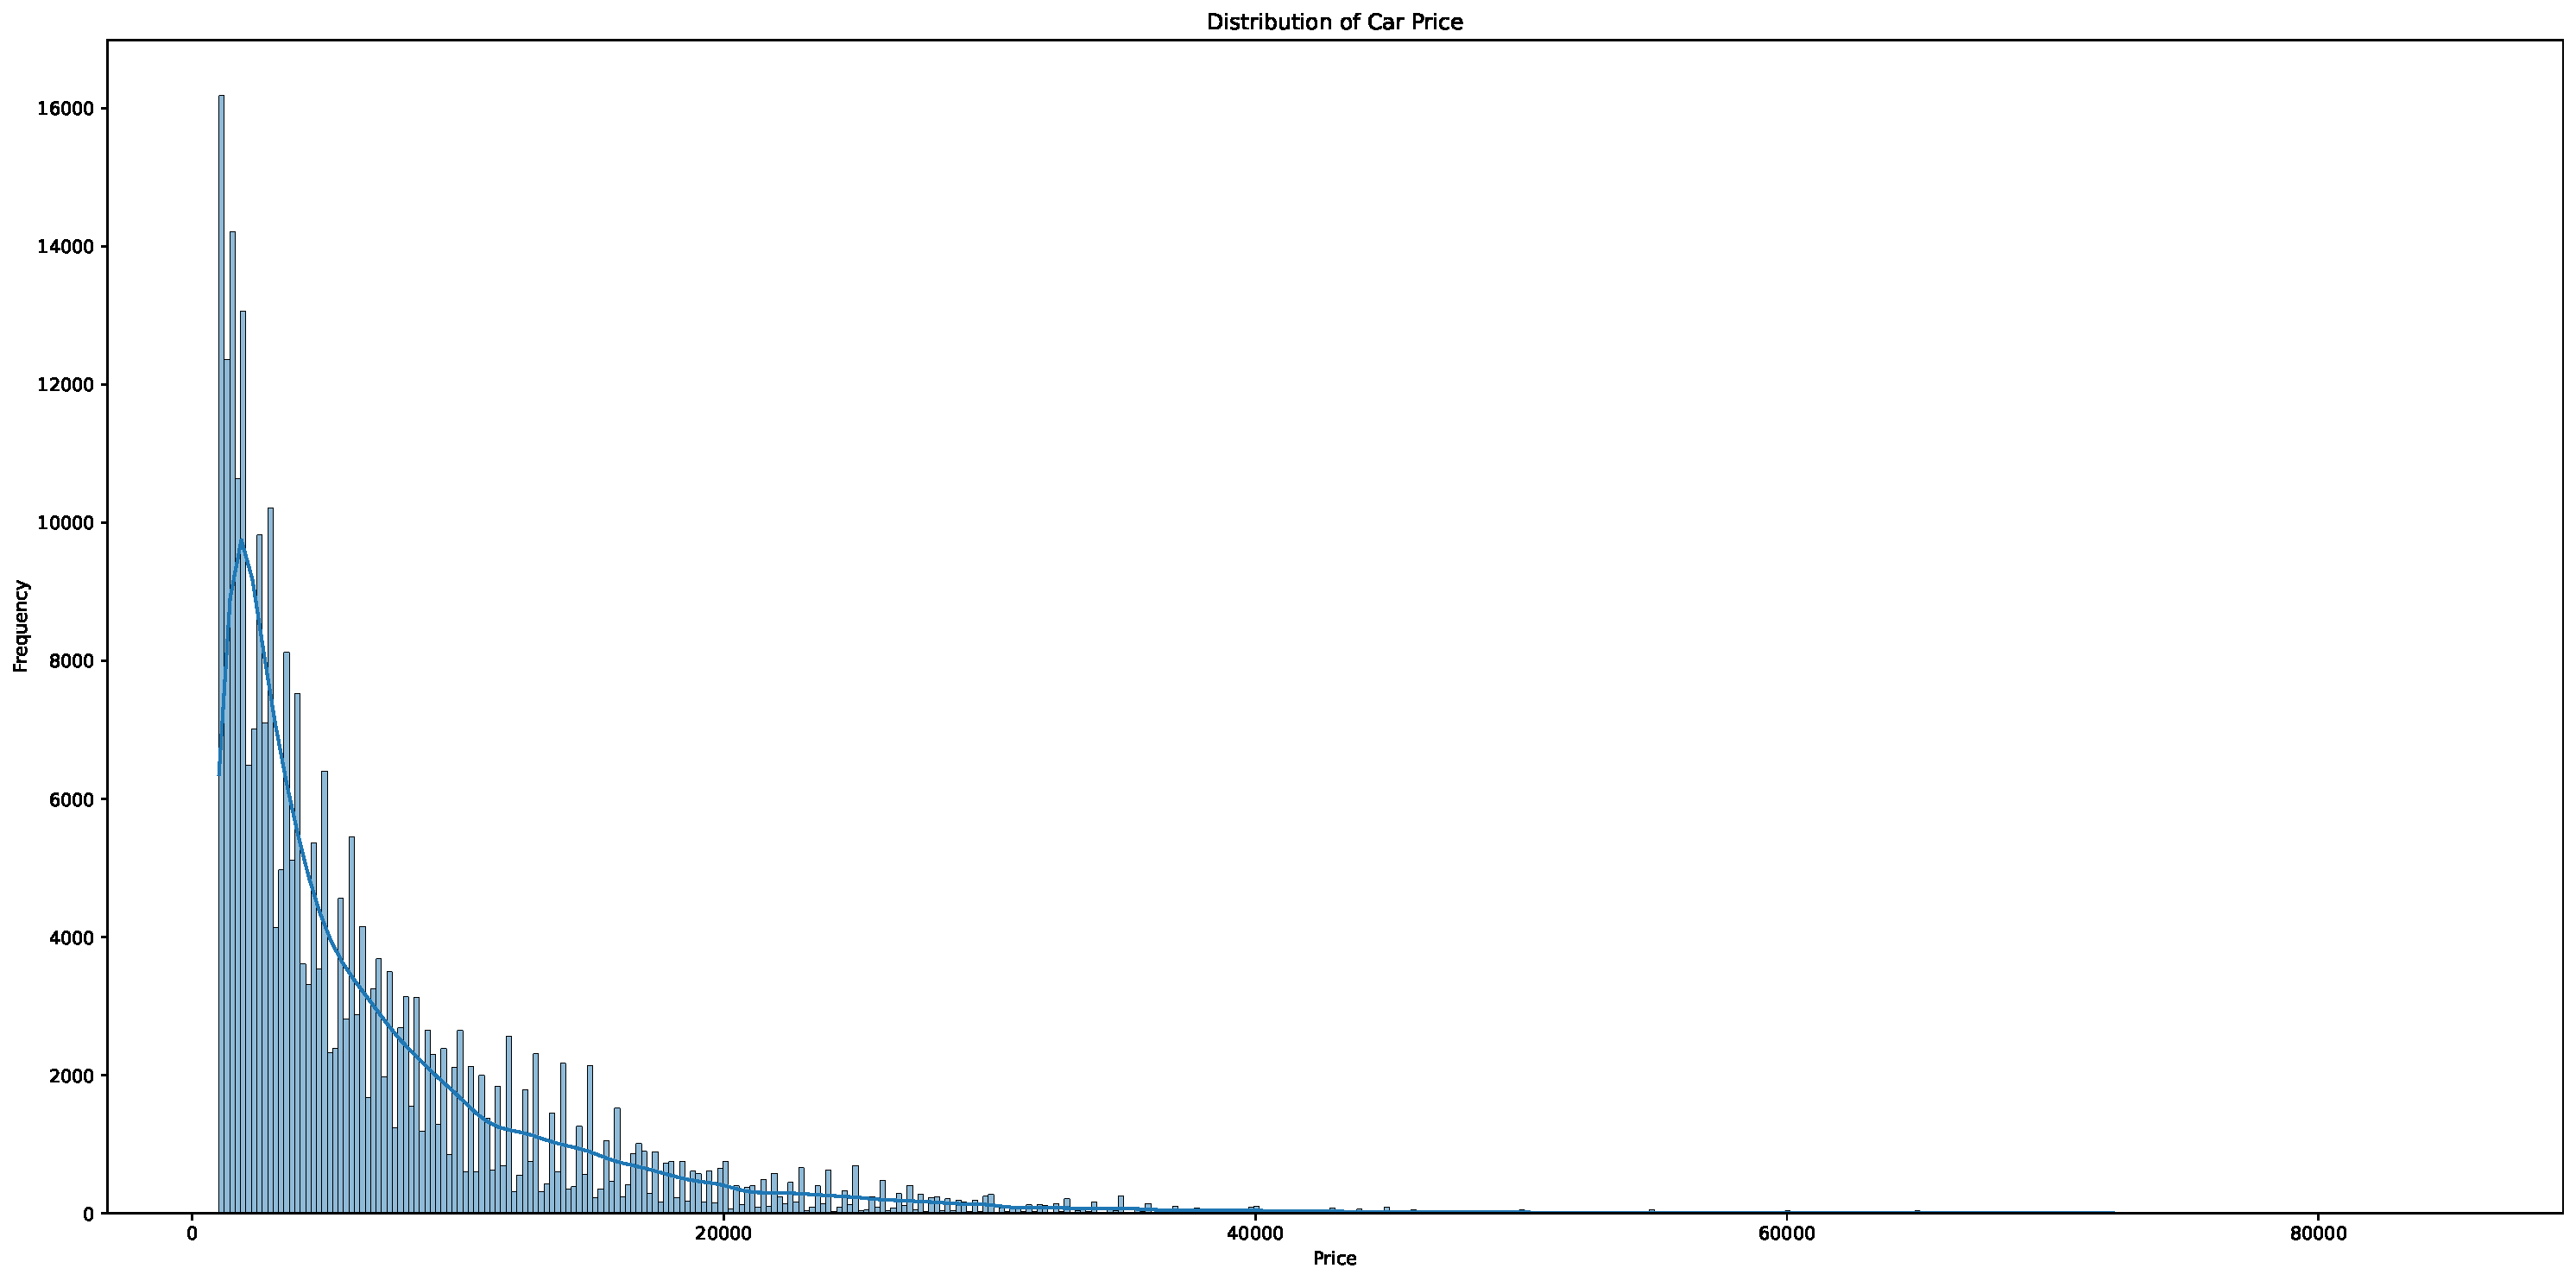
\includegraphics[trim=0 0 6cm 0, clip, width=\linewidth]{figures/car_price_distribution.pdf}
\caption{Distribution of car prices in the dataset(whole graph is not shown)}
\label{fig:car_price_dist}
\end{figure}

Our plot showcases that we have rather a lot of extreme outliers. We can also
assume that the price distribution is not 'normal' and it is skewed. An
assumption that we confirm by running various normality tests such as
'Anderson-Darling', 'Kolmogorov-Smirnov', 'Jarque-Bera' and others. In addition
the skeweness of the distribution is found to be `5.13`, which confirms that our
distribution is extremely right skewed.

\subsubsection{Categorical Features}
We start examining our target variable. This is the distribution of Car Prices:

\begin{figure}[H]
\centering
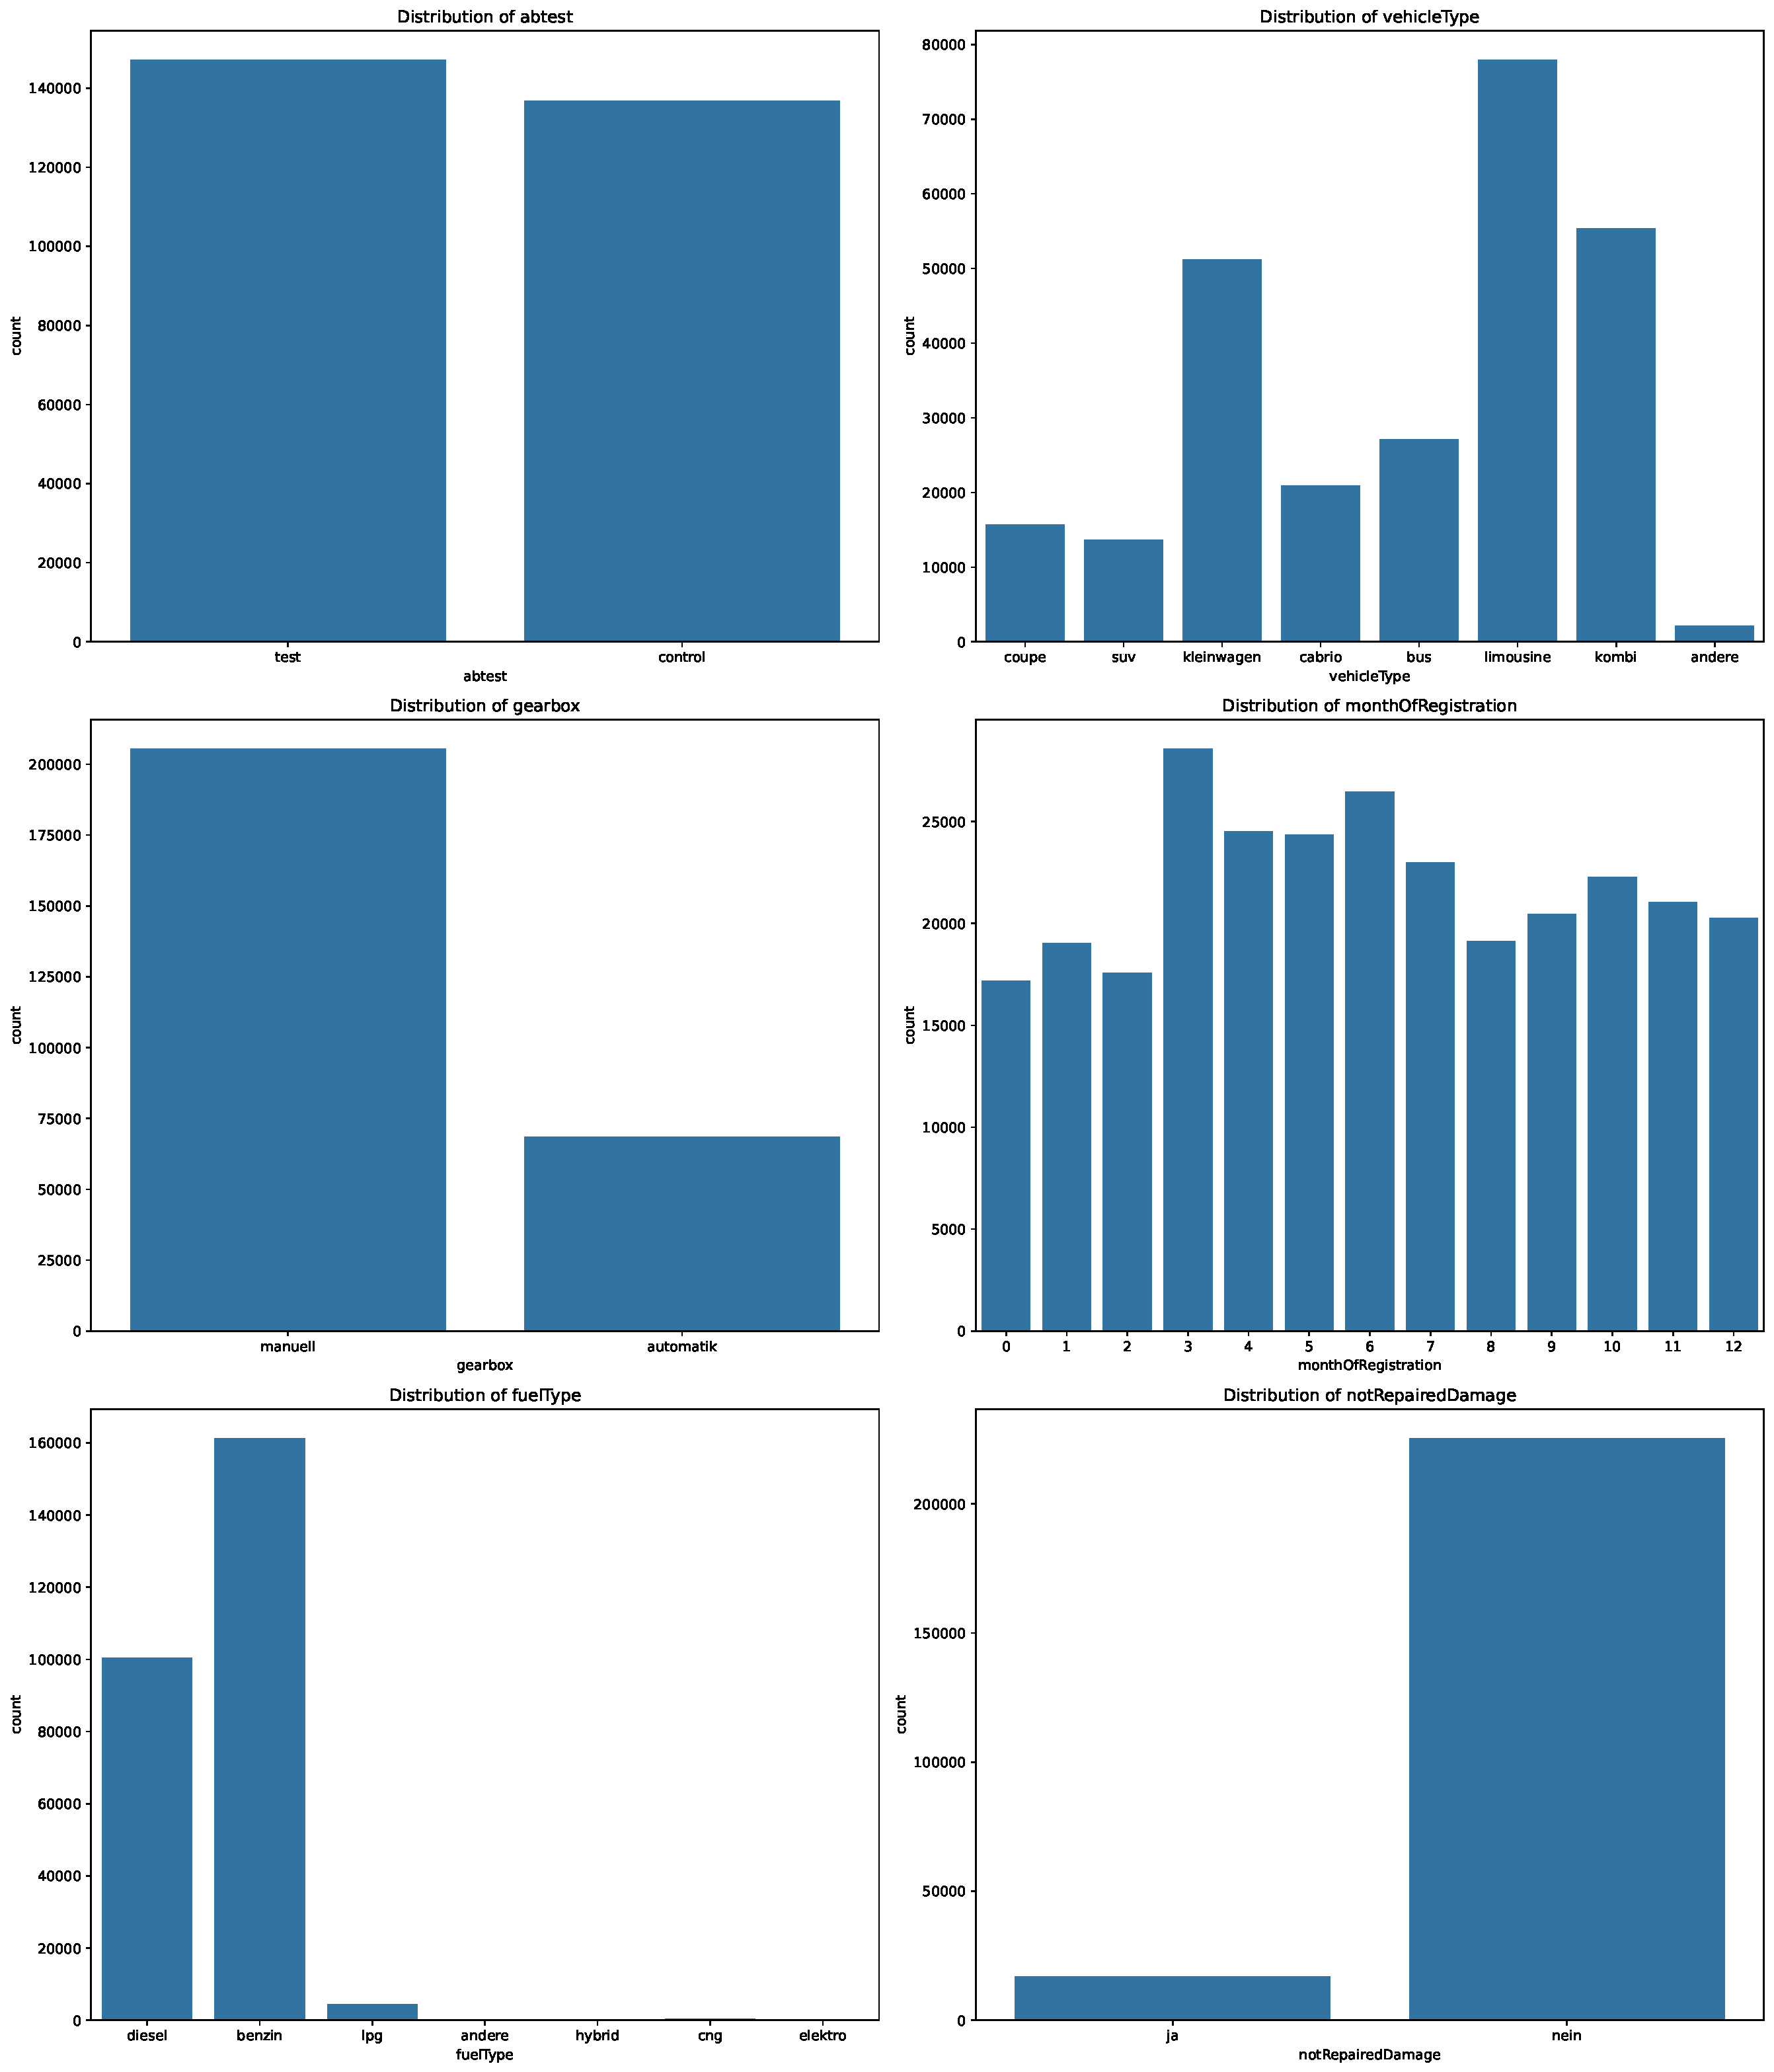
\includegraphics[width=\linewidth]{figures/cat_features_distribution.pdf}
\caption{Distribution of Categorical features in the dataset}
\label{fig:cat_features_dist}
\end{figure}

\begin{enumerate}
    \item \textbf{ABtest (abtest)}
    \begin{itemize}
        \item Both the \textit{test} and \textit{control} groups are similarly
                distributed, with the \textit{test} group appearing slightly
                more frequently.
        \item This feature may be valuable for analyzing the impact of A/B
                testing on vehicle pricing.
    \end{itemize}
    
    \item \textbf{Vehicle Type (vehicleType)}
    \begin{itemize}
        \item The distribution is dominated by three types:
                \textit{kleinwagen}, \textit{limousine}, and \textit{kombi}.
        \item Other types still appear frequently enough to be considered relevant.
        \item The \textit{andere} category is underrepresented and may benefit
                from oversampling during model training.
    \end{itemize}
    
    \item \textbf{Gearbox (gearbox)}
    \begin{itemize}
        \item Most vehicles have a manual (\textit{manuell}) gearbox, although
                a significant number are automatic (\textit{automatik}).
        \item Gearbox type could be an important predictor of vehicle price.
    \end{itemize}
    
    \item \textbf{Month of Registration (monthOfRegistration)}
    \begin{itemize}
        \item Car registrations are relatively evenly distributed across the months.
        \item The presence of a value like 0 or 13 suggests potential
                placeholder values for missing or erroneous data, though the
                dataset documentation does not clarify this.
    \end{itemize}
    
    \item \textbf{Fuel Type (fuelType)}
    \begin{itemize}
        \item \textit{Benzin} is by far the most common fuel type.
        \item \textit{Diesel} also appears frequently enough to influence modeling.
        \item Less common fuel types—such as \textit{lpg}, \textit{hybrid},
                \textit{cng}, \textit{elektro}, and \textit{andere}—occur too
                infrequently and might be better grouped into a single
                \texttt{other} category.
    \end{itemize}

    \item \textbf{Unrepaired Damage (notRepairedDamage)}
    \begin{itemize}
        \item The majority of entries report \textit{nein} (no damage).
        \item A smaller portion reports \textit{ja} (damage present), which
                could still provide useful information during training.
    \end{itemize}
\end{enumerate}

\begin{figure}[H]
\centering
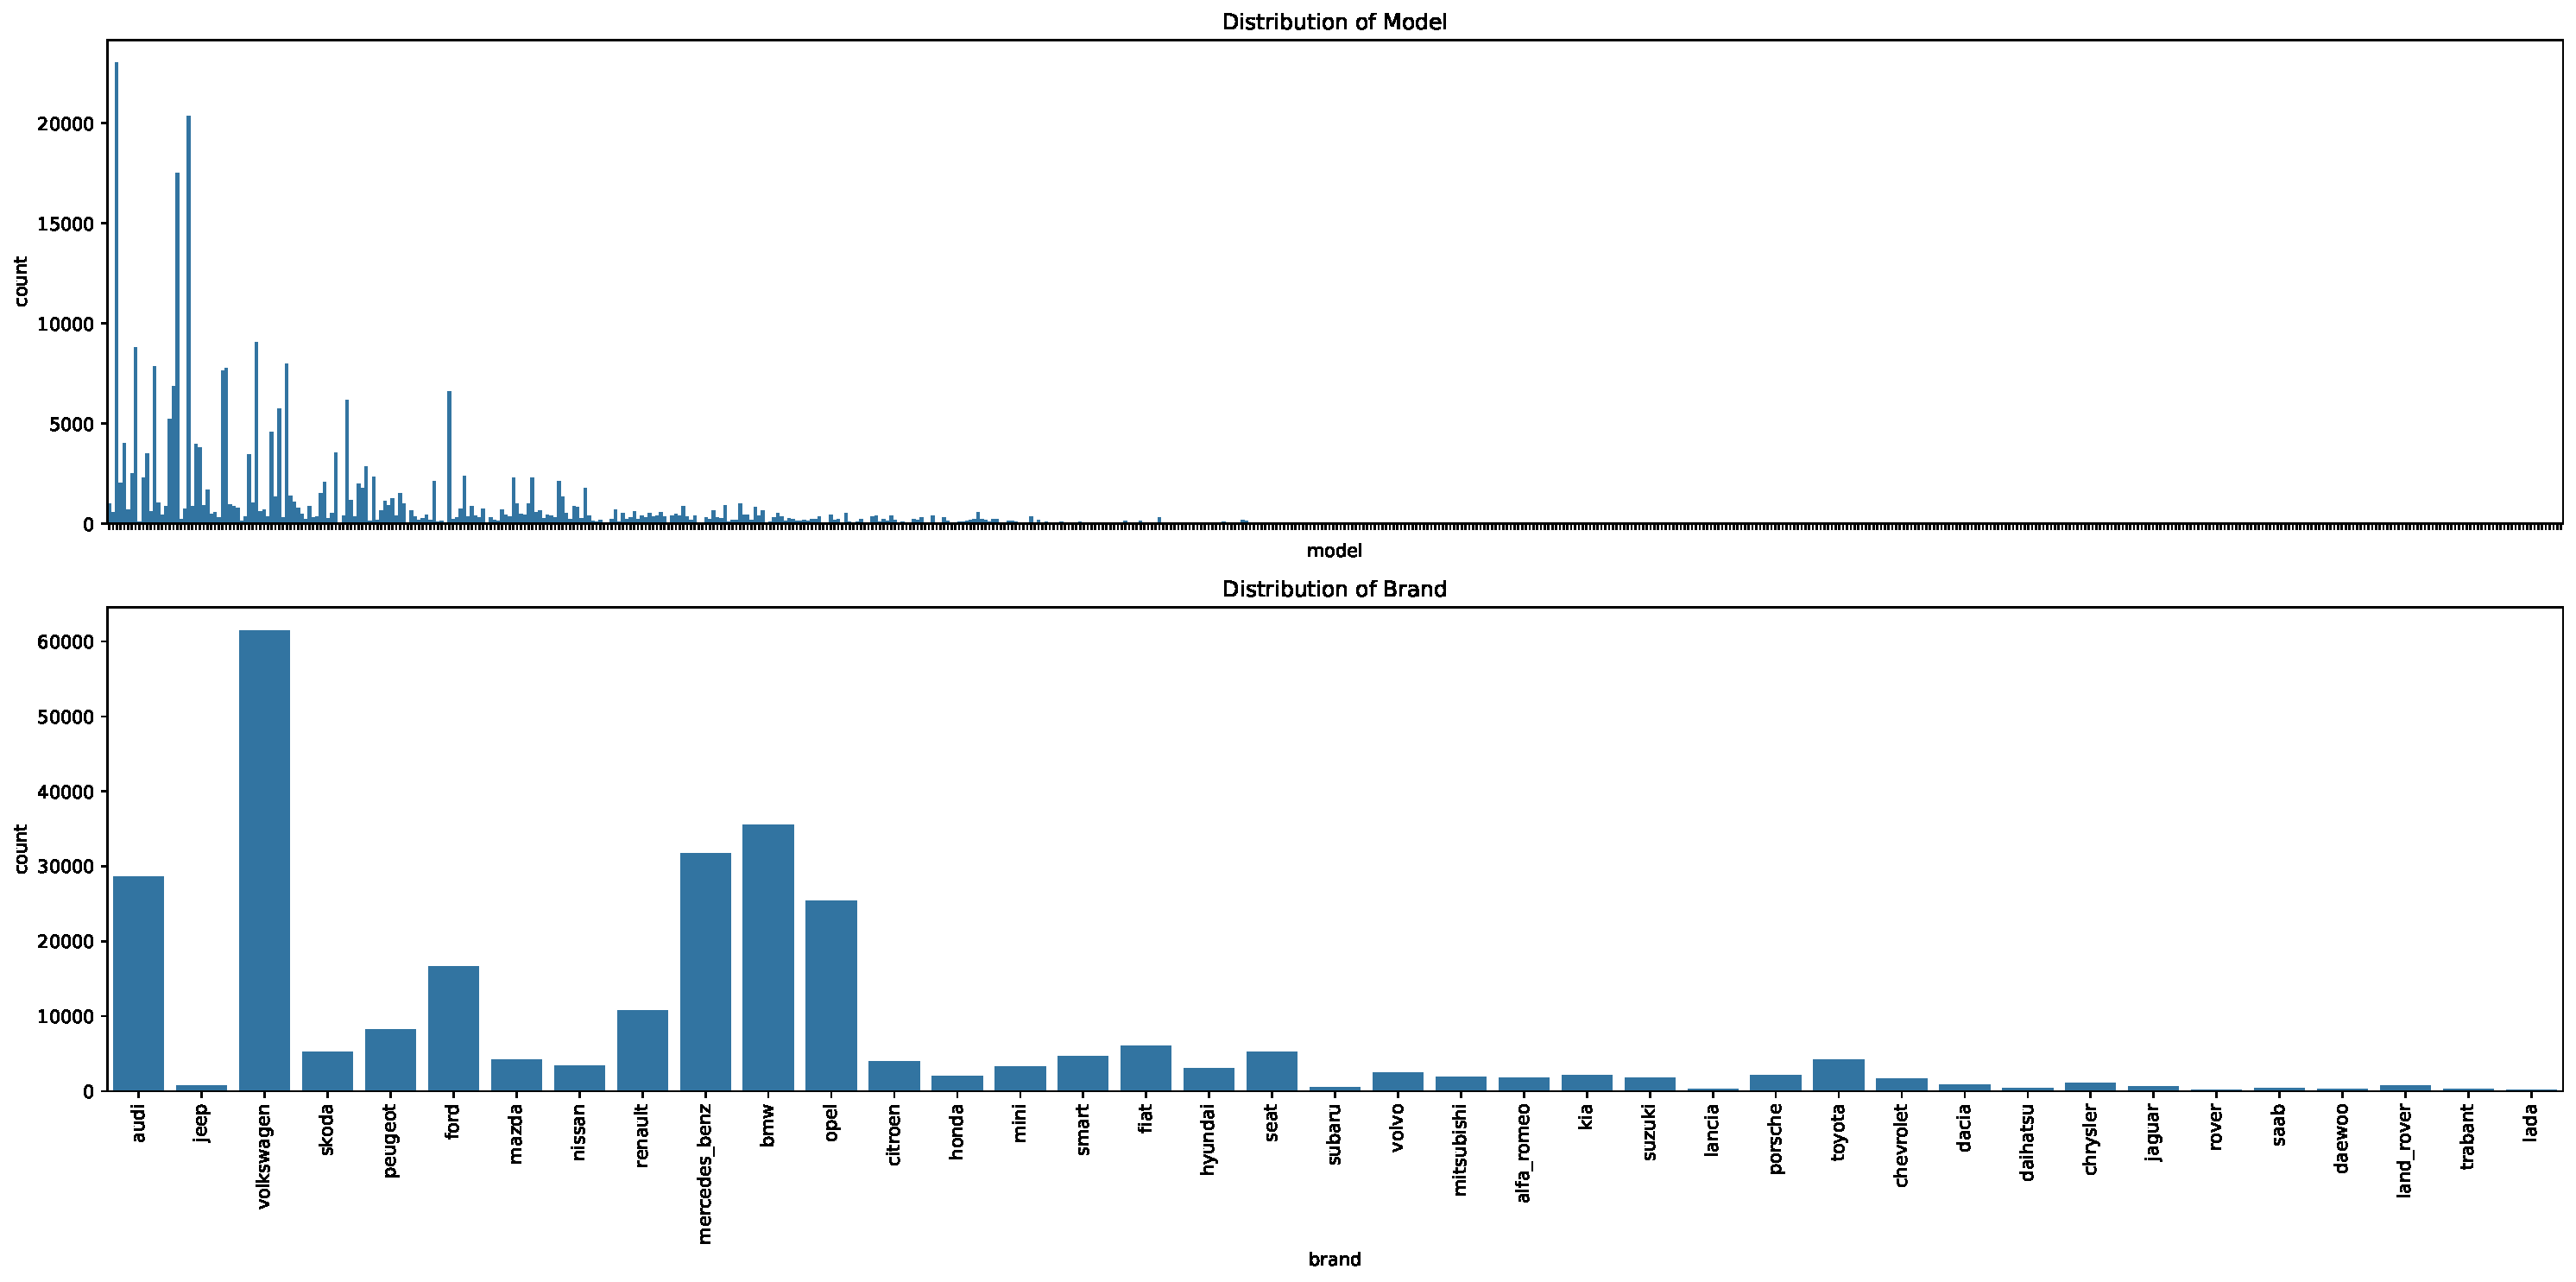
\includegraphics[trim=0 0 10cm 0, clip, width=\linewidth]{figures/model_brand_distribution.pdf}
\caption{Distribution of Model and Brand features in the dataset (whole graph
is not shown)}
\label{fig:model_brand_dist}
\end{figure}

Both 'model' and 'brand' are categorical with a very large amount of possible
values, dealing with these columns might prove difficult.

\begin{figure}[H]
\centering
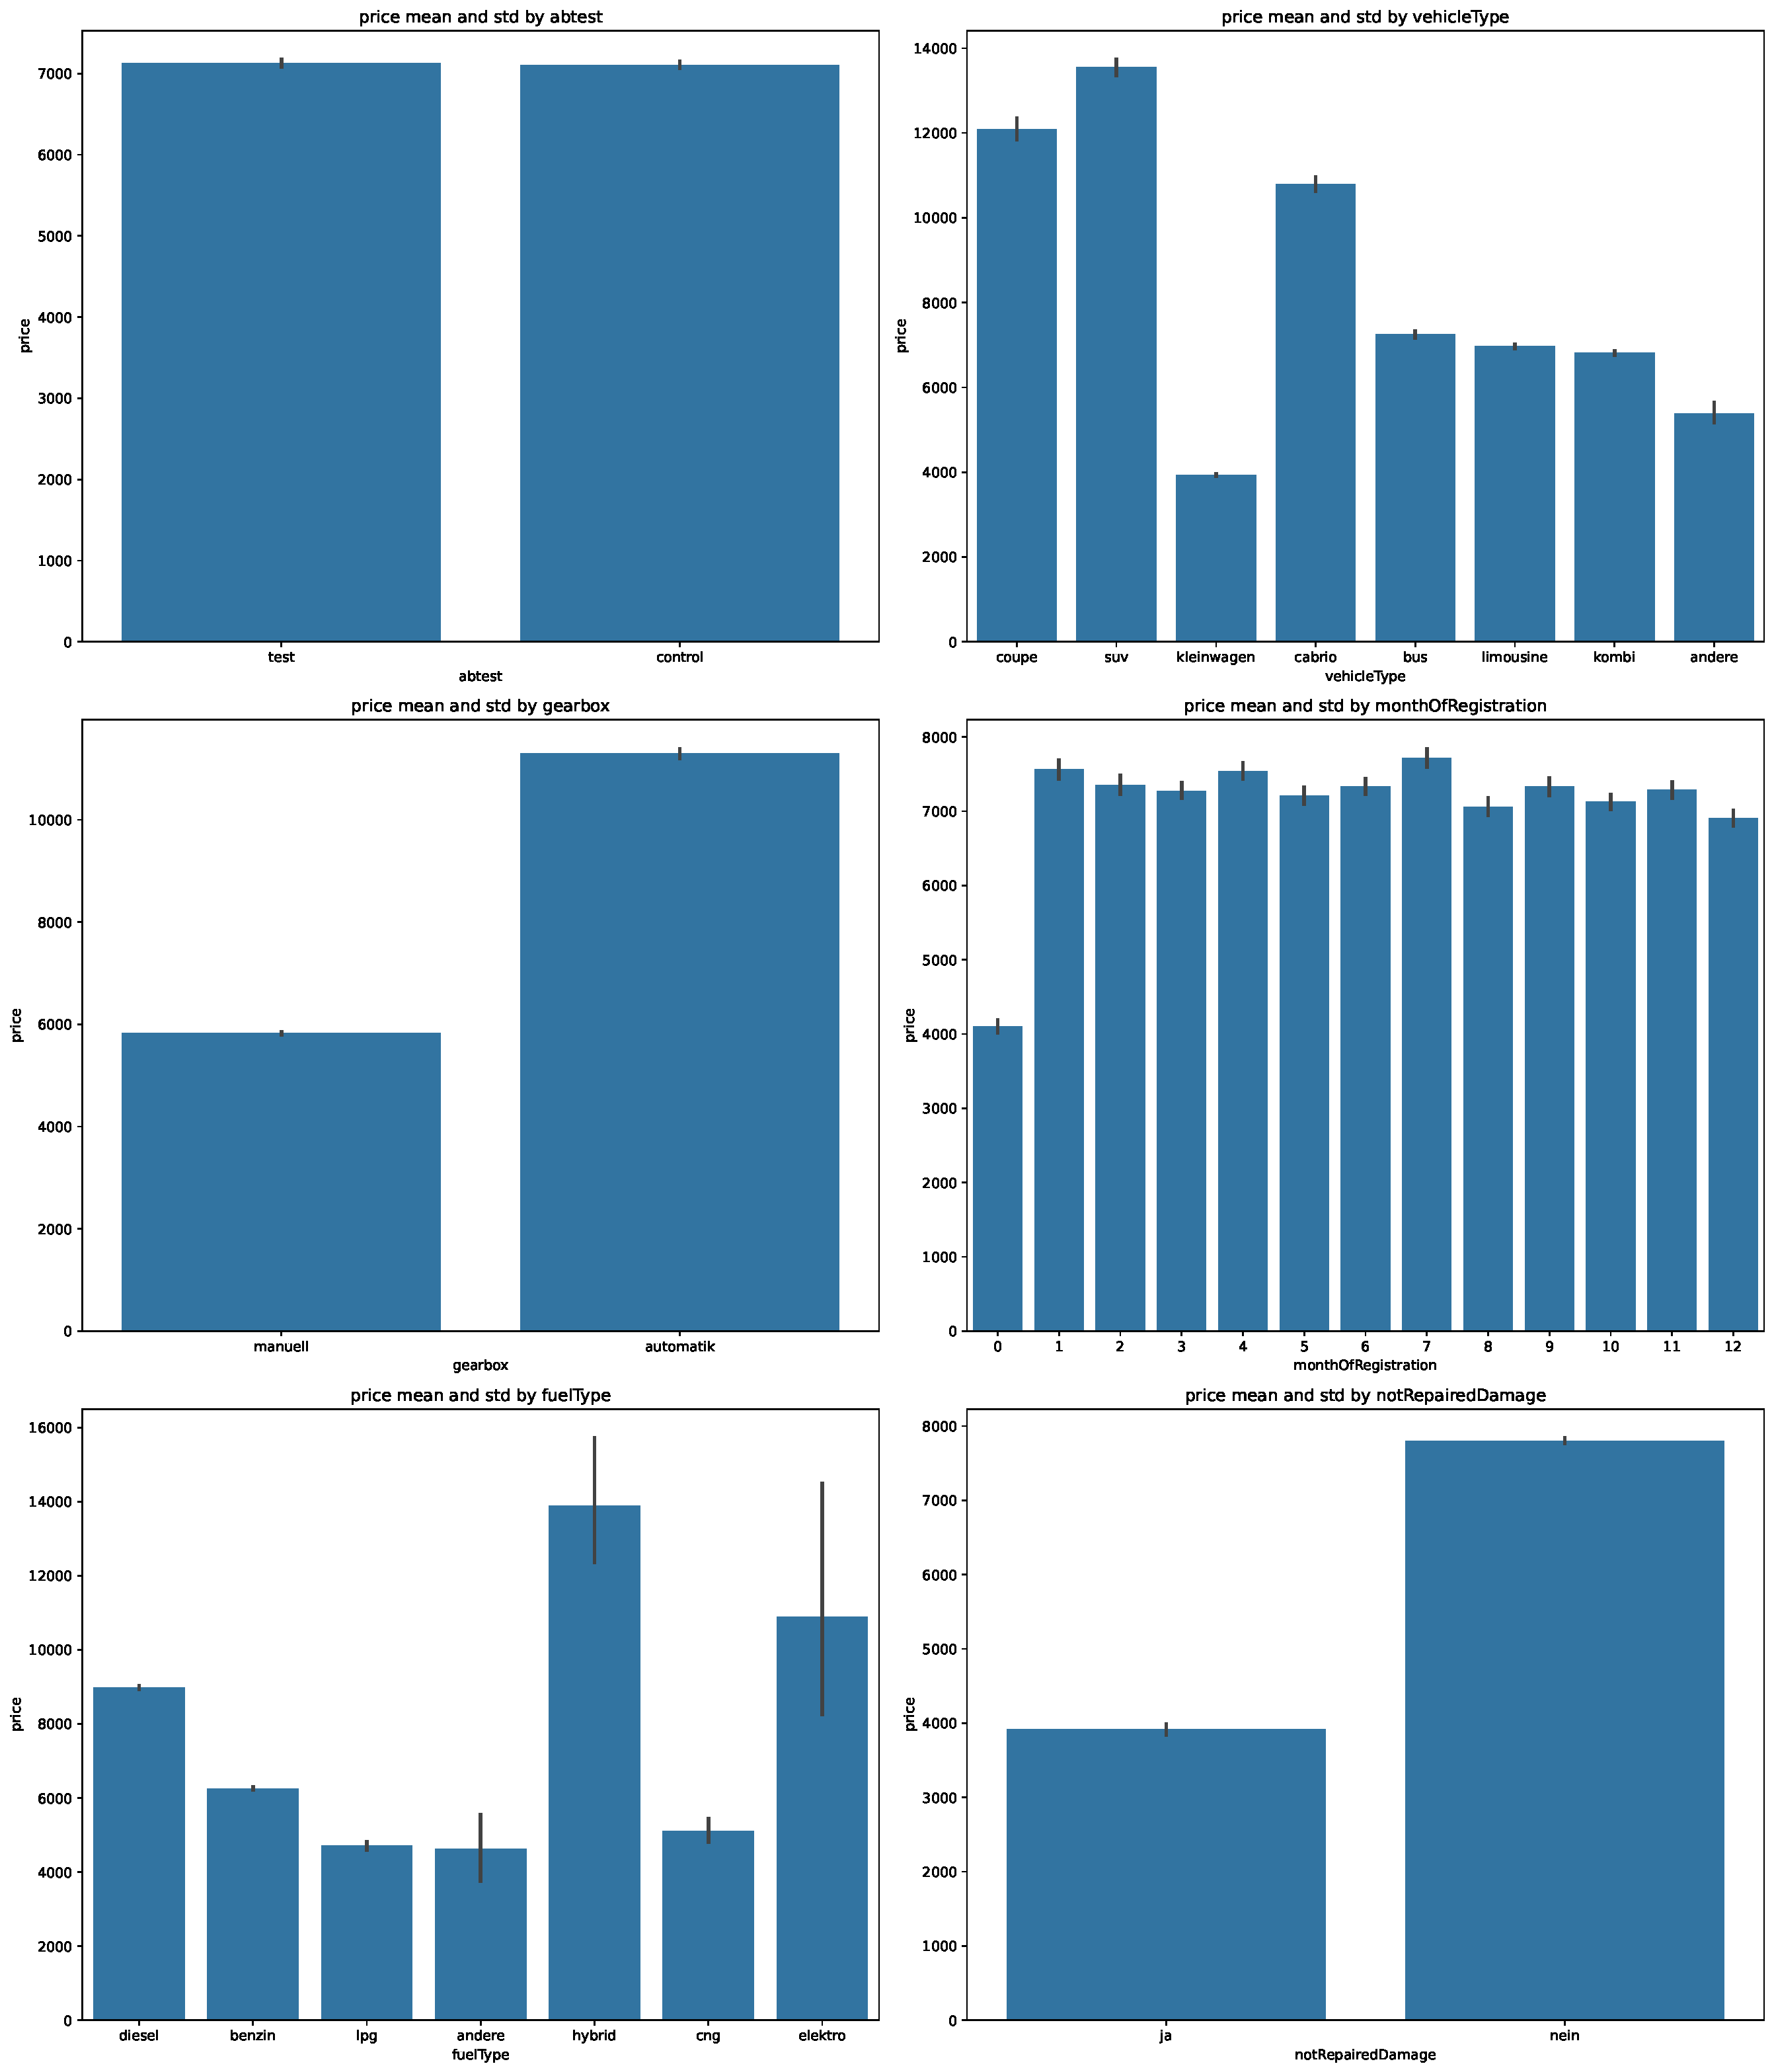
\includegraphics[width=\linewidth]{figures/cat_features_barplot.pdf}
\caption{Target mean and std by categorical features}
\label{fig:cat_features_barplot}
\end{figure}

\vspace{1em}
\noindent\textbf{General Observations:}
\begin{itemize}
    \item Most correlations identified align with our expectations and provide
            strong signals for price prediction.
    \item The behavior of the \texttt{monthOfRegistration} feature,
            particularly the \texttt{0} value, remains unclear and requires
            further clarification.
\end{itemize}

\begin{enumerate}
    \item \textbf{ABtest (abtest)}
    \begin{itemize}
        \item Both categories of \texttt{abtest} exhibit nearly identical average prices.
        \item This suggests that the feature has no meaningful correlation with the target variable.
        \item Given its apparent lack of influence, it may be beneficial to
                remove this feature from the model.
    \end{itemize}

    \item \textbf{Type of Vehicle (vehicleType)}
    \begin{itemize}
        \item Each vehicle category shows a distinct average price, though with
                relatively small variance.
        \item This indicates a moderate correlation between vehicle type and
                price, supporting its inclusion as a predictive feature.
    \end{itemize}

    \item \textbf{Gearbox (gearbox)}
    \begin{itemize}
        \item The average price differs substantially between gearbox types.
        \item This strong association implies high predictive value for this
                feature.
    \end{itemize}

    \item \textbf{Month of Registration (monthOfRegistration)}
    \begin{itemize}
        \item Most months yield similar mean prices.
        \item However, entries labeled as month \texttt{0} differ
                significantly, warranting further investigation to understand
                whether this represents missing data or another issue.
    \end{itemize}

    \item \textbf{Fuel Type (fuelType)}
    \begin{itemize}
        \item The fuel type shows a strong correlation with vehicle price, as
                different categories yield significantly different averages.
        \item Categories such as \textit{hybrid} and \textit{elektro} should
                not be grouped into an \texttt{other} category due to their
                distinct pricing patterns.
        \item It may be worth discussing whether to retain or exclude
                low-frequency categories like \textit{hybrid} and
                \textit{elektro} depending on modeling objectives.
        \item Less frequent types such as \textit{lpg}, \textit{andere}, and
                \textit{cng} could potentially be grouped into an
                \texttt{other} category.
    \end{itemize}

    \item \textbf{Unrepaired Damage (notRepairedDamage)}
    \begin{itemize}
        \item A strong correlation exists between the presence of unrepaired
                damage and lower prices.
        \item This suggests high predictive value for this feature.
    \end{itemize}
\end{enumerate}

\begin{figure}[H]
\centering
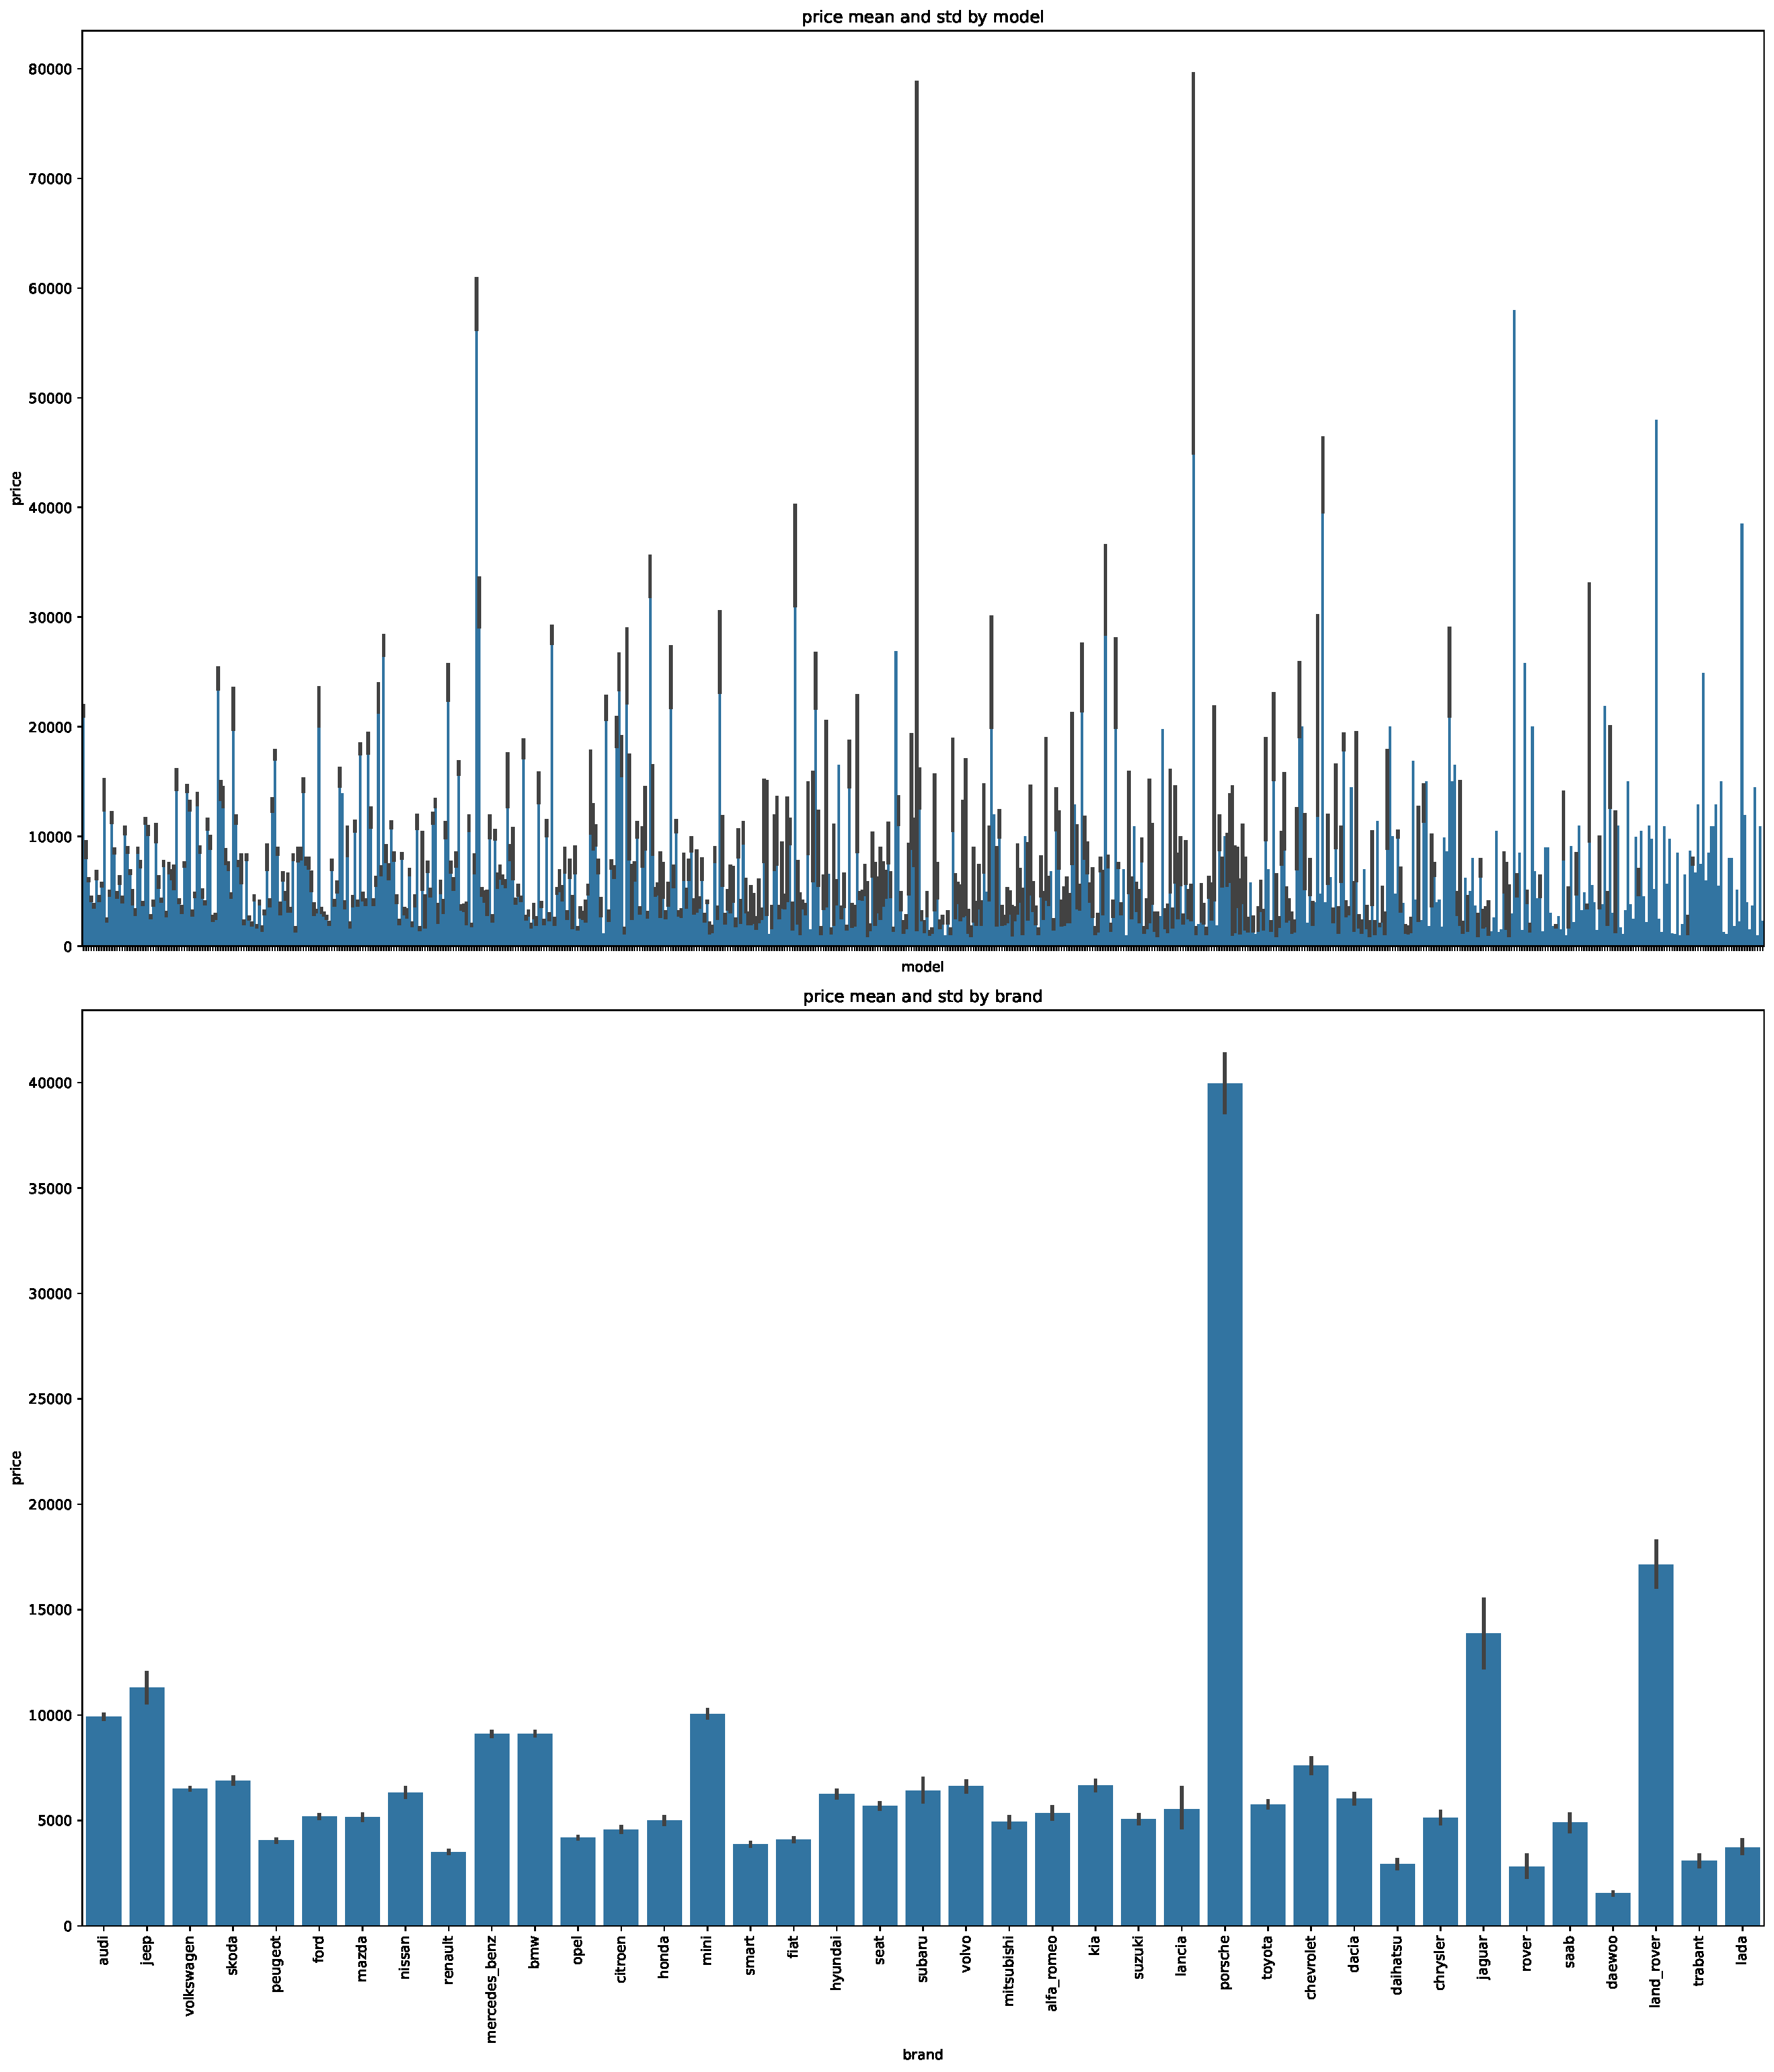
\includegraphics[trim=0 0 10cm 0, clip,width=\linewidth]{figures/model_brand_barplot.pdf}
\caption{Target mean and std by model and brand features}
\label{fig:model_brand_barplot}
\end{figure}

\begin{enumerate}
    \item \textbf{Model (model)}
    \begin{itemize}
        \item The \texttt{model} feature shows a strong correlation with
                \texttt{price}.
        \item Many models exhibit high variance in price, indicating that this
                feature captures a wide range of vehicle characteristics.
        \item Different models within the same brand often have significantly
                different price points. For example, both the \texttt{911} and
                \texttt{Cayenne} belong to Porsche, yet target different
                segments with distinct pricing.
    \end{itemize}

    \item \textbf{Brand (brand)}
    \begin{itemize}
        \item The \texttt{brand} feature also shows a strong correlation with
                \texttt{price}.
        \item While most brands show relatively low variation in price, a few
                have high deviation, which may merit further investigation.
    \end{itemize}
\end{enumerate}

\vspace{1em}
\noindent\textbf{General Observations:}
\begin{itemize}
    \item Variability within a brand’s price distribution may be explained by
            the diversity of models it offers.
    \item Even within the same model, vehicles may differ in important
            ways—such as damage status, age, or other correlated features—that
            contribute to price outliers.
    \item Outliers are present in most brands and models, with some categories
            exhibiting more extreme deviations than others.
\end{itemize}

\begin{table}[H]
\centering
\resizebox{\linewidth}{!}{%
\begin{tabular}{lll}
\toprule
name & model & brand \\
\midrule
Golf\_3\_1.6 & golf & volkswagen \\
A5\_Sportback\_2.7\_Tdi & NaN & audi \\
Jeep\_Grand\_Cherokee\_"Overland" & grand & jeep \\
GOLF\_4\_1\_4\_\_3TÜRER & golf & volkswagen \\
Skoda\_Fabia\_1.4\_TDI\_PD\_Classic & fabia & skoda \\
BMW\_316i\_\_\_e36\_Limousine\_\_\_Bastlerfahrzeug\_\_Export & 3er & bmw \\
Peugeot\_206\_CC\_110\_Platinum & 2\_reihe & peugeot \\
VW\_Derby\_Bj\_80\_\_Scheunenfund & andere & volkswagen \\
Ford\_C\_\_\_Max\_Titanium\_1\_0\_L\_EcoBoost & c\_max & ford \\
VW\_Golf\_4\_5\_tuerig\_zu\_verkaufen\_mit\_Anhaengerkupplung & golf & volkswagen \\
\bottomrule
\end{tabular}
}
\caption{Sample of car name, model, and brand from dataset}
\label{tab:car_name}
\end{table}

A difficulty arises when dealing with the feature 'name'. As shown from the
Table~\ref{tab:car_name}, each value is distinct and does not follow any
specific convention. This is important since 'model' can be derived from 'name'
and model has 12,148 missing values. We manage to derive the model of the cars
from their name by applying fuzzy match of the name into known models of the
corresponding brand. This is important since the price of a car within the same
brand can vary largely due to the specific model, as shown here 

\subsubsection{Numerical Features}
Distributions of numerical features follow.
\begin{figure}[H]
\centering
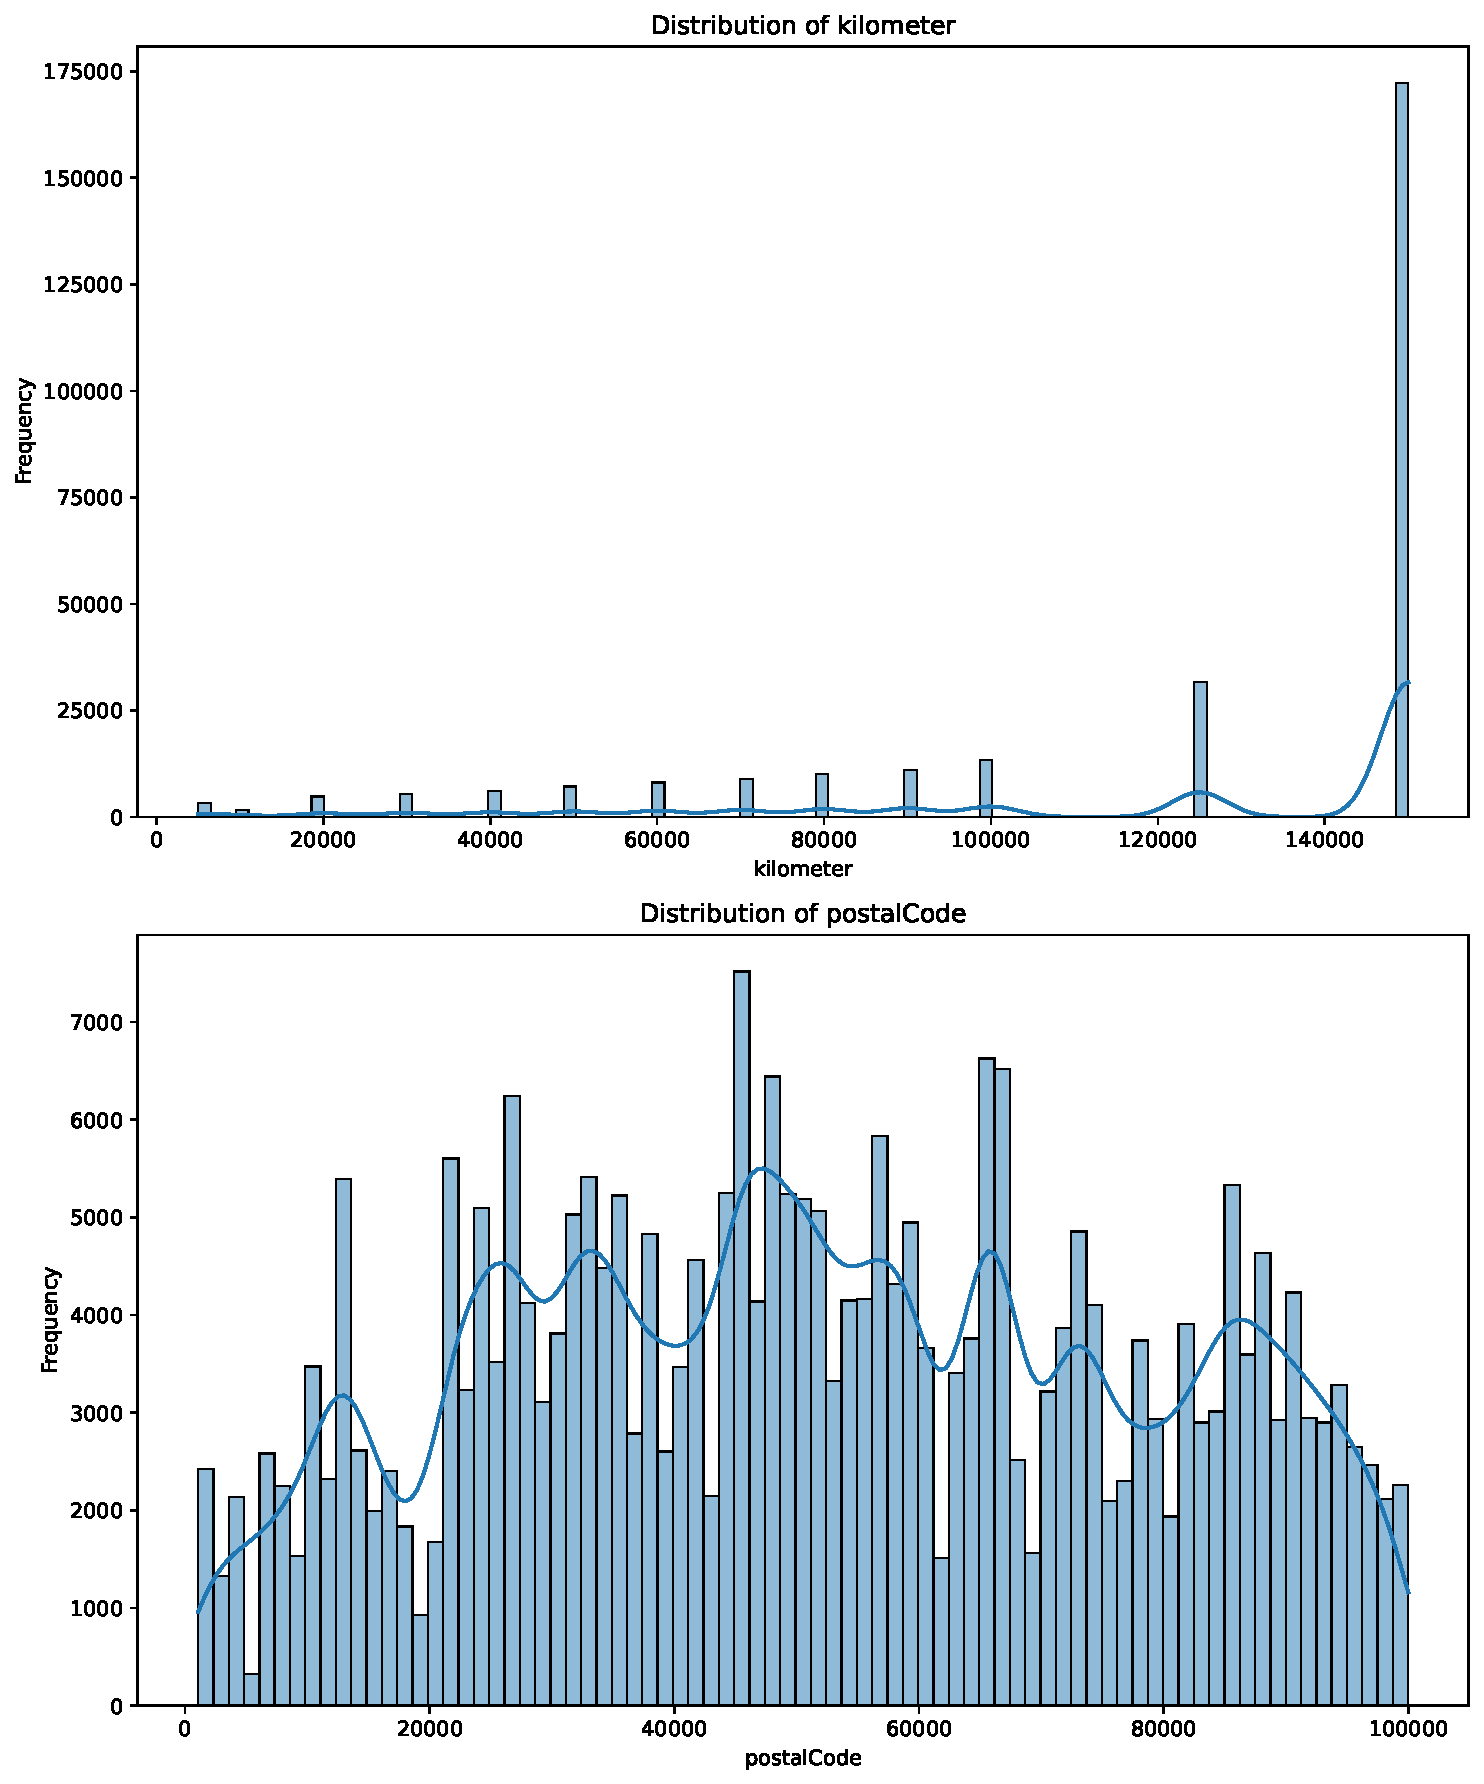
\includegraphics[width=\linewidth]{figures/kilometer_postalCode_distribution.pdf}
\caption{Distribution of numerical features}
\label{fig:kilometer_postalCode_dist}
\end{figure}

\begin{figure}[H]
\centering
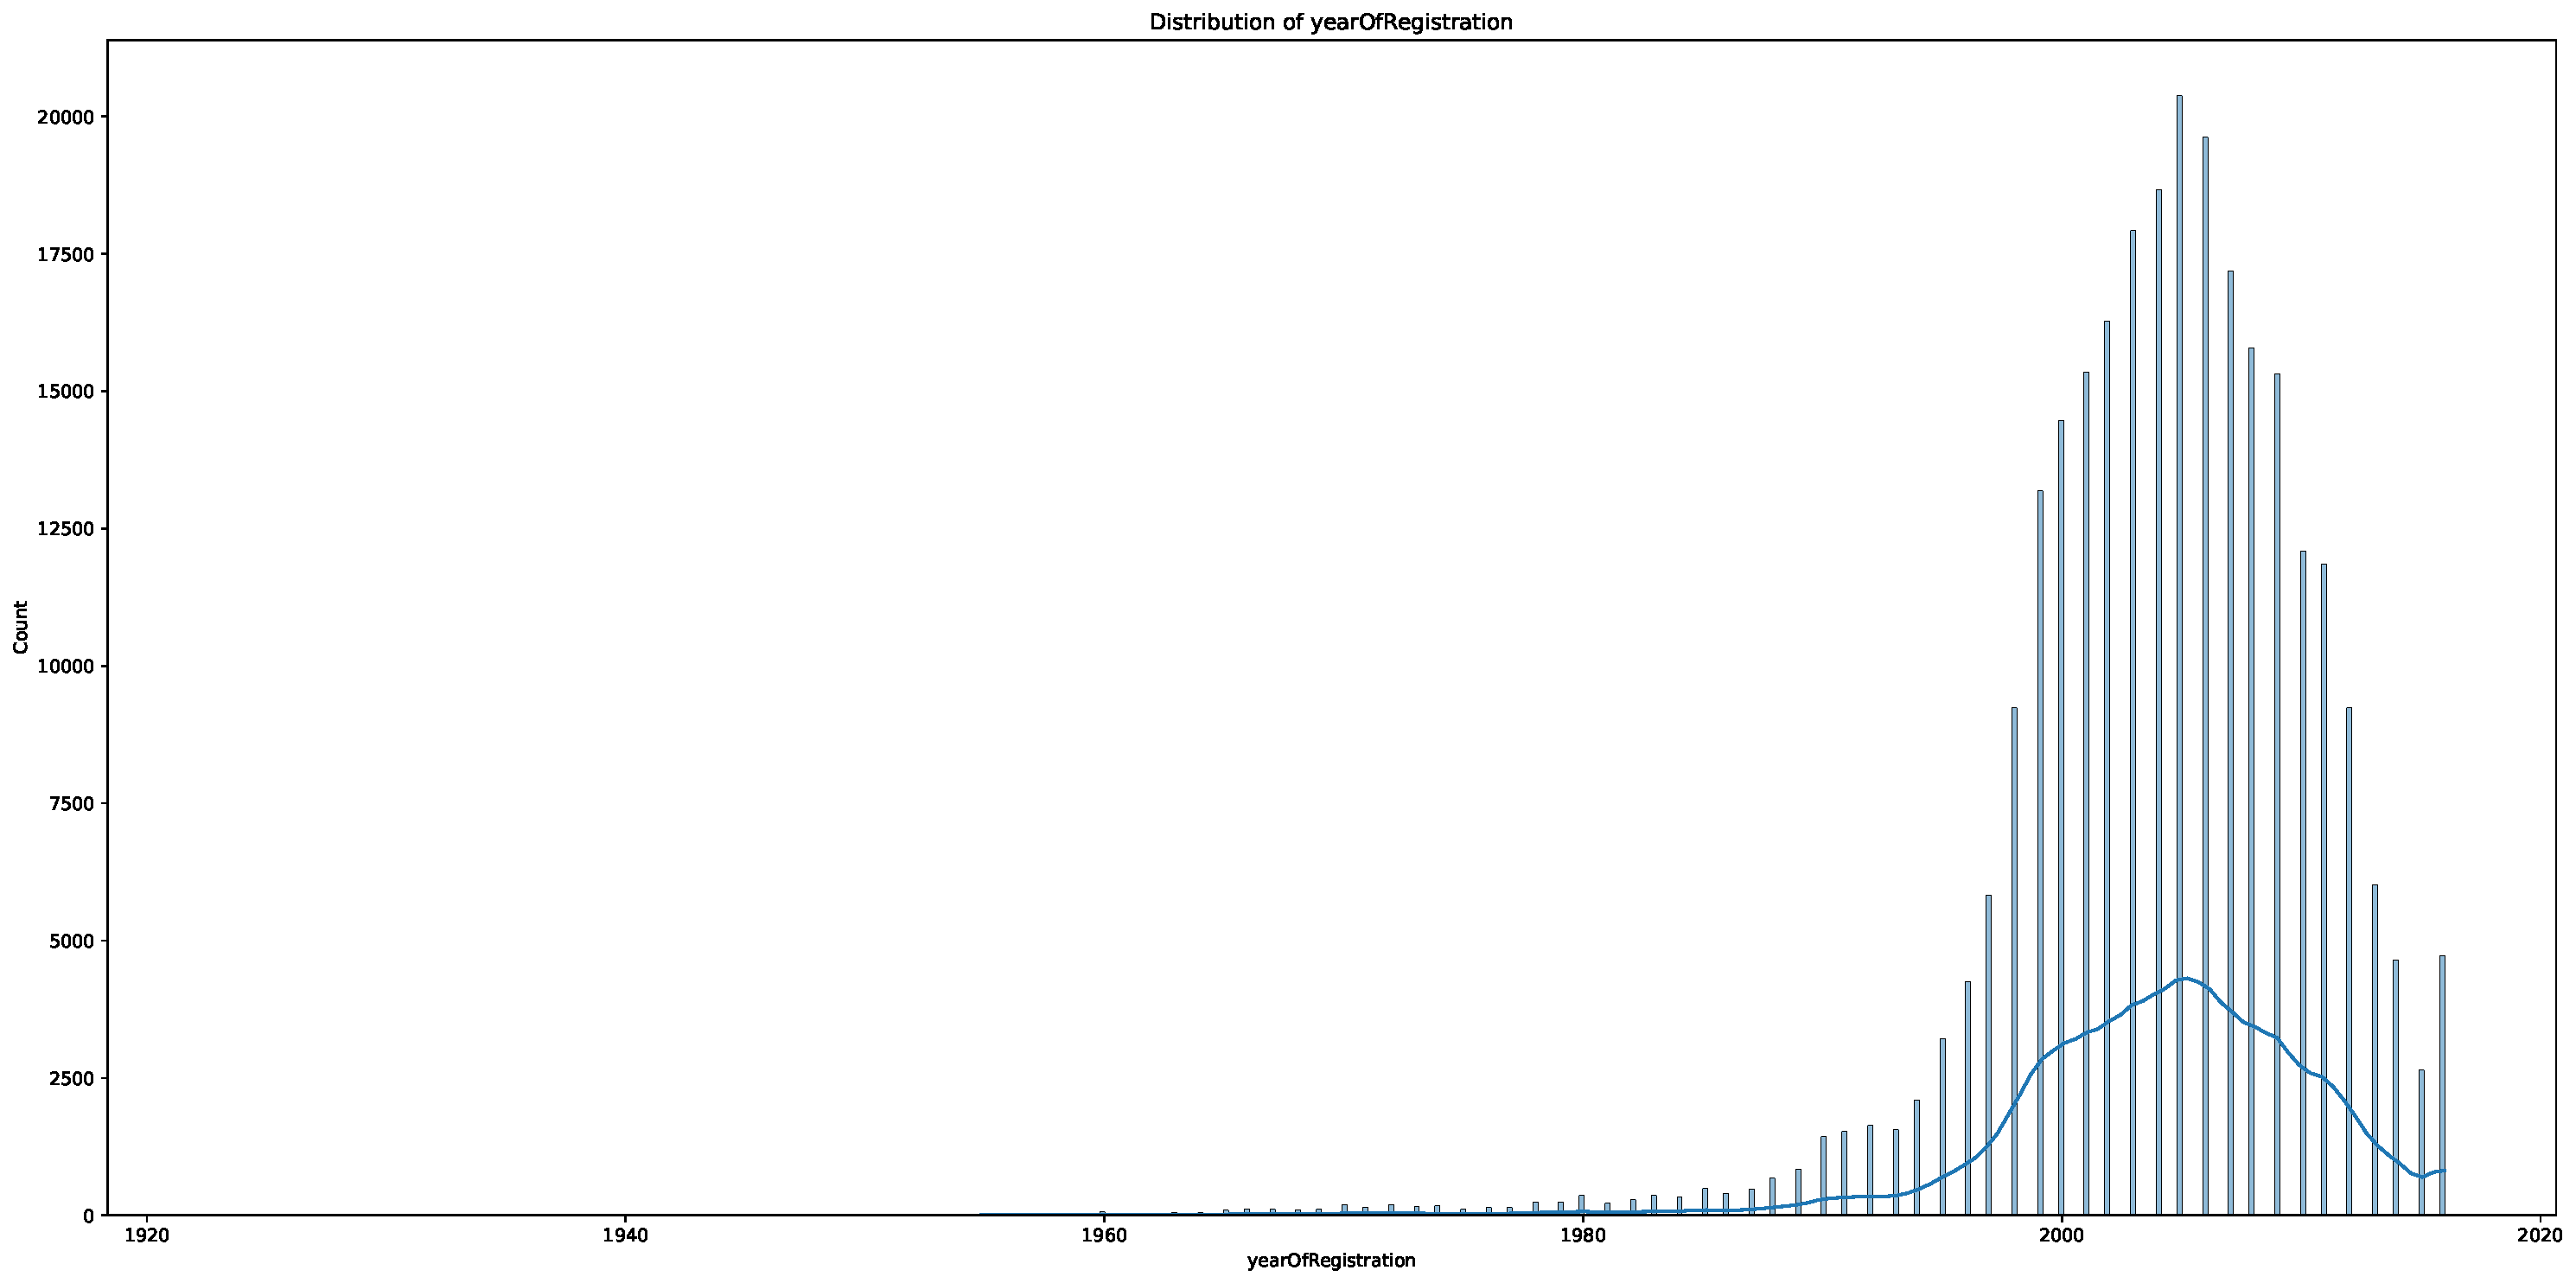
\includegraphics[width=\linewidth]{figures/yearOfRegistration_distribution.pdf}
\caption{Distribution of yearOfRegistration}
\label{fig:yearOfRegistration_dist}
\end{figure}

\begin{figure}[H]
\centering
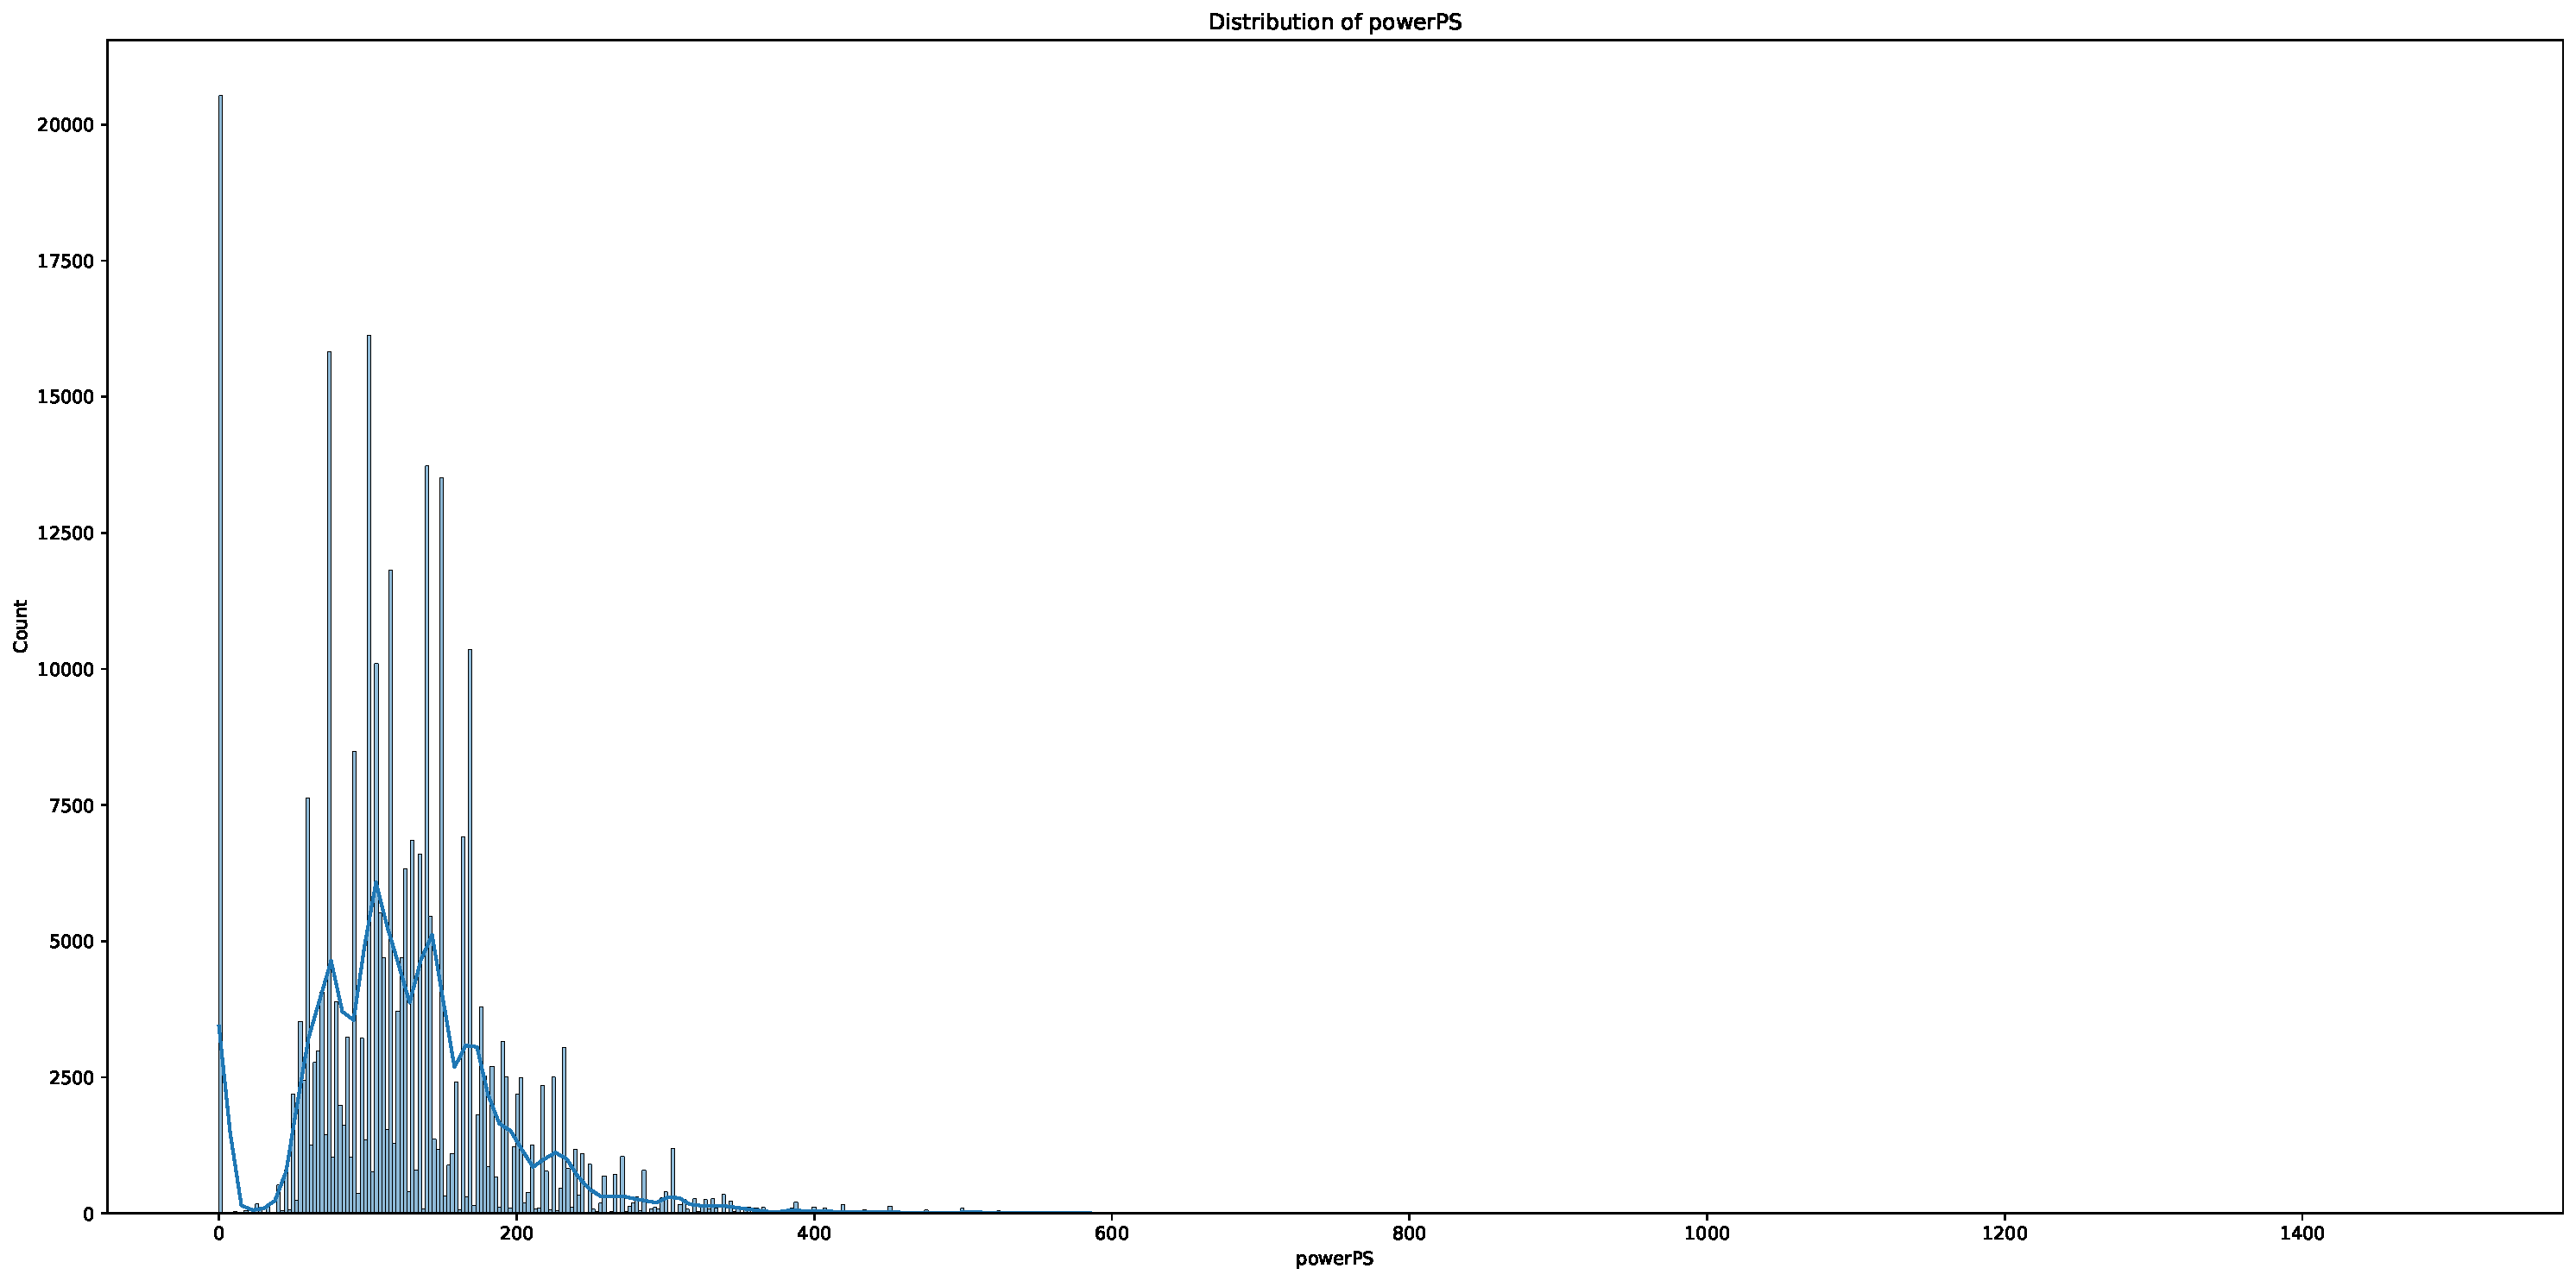
\includegraphics[width=\linewidth]{figures/powerPS_distribution.pdf}
\caption{Distribution of powerPS}
\label{fig:powerPS_dist}
\end{figure}

Every feature except 'postalCode' is largely-extremely skewed, and no feature
follows normal distribution. It needs to be stated that 'yearOfRegistration'
and 'powerPS' had a large number of erroneous values. For example dozens of
rows had 'yearOfRegistration' values less than 1920 or greater than 2016
(dataset was collected in 2016) and 'powerPS' had values greater than 1500.

\begin{figure}[H]
\centering
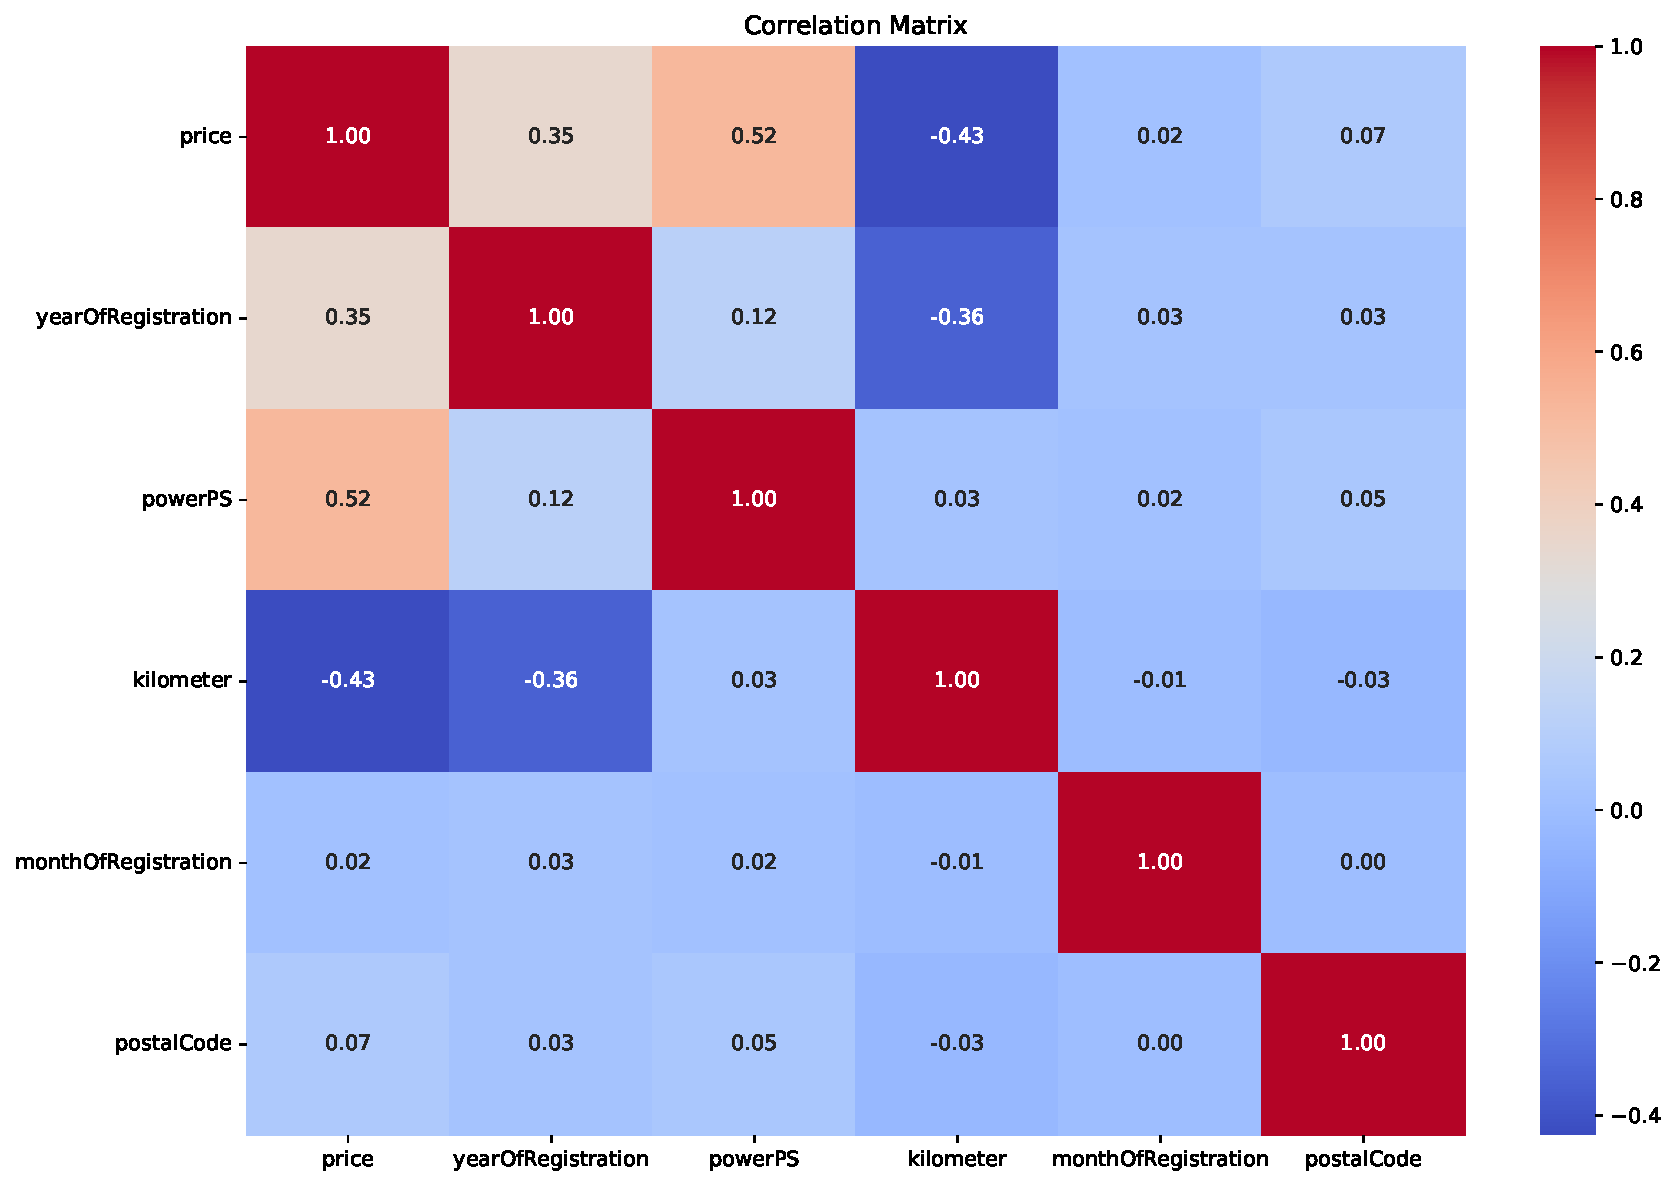
\includegraphics[width=\linewidth]{figures/heatmap.pdf}
\caption{Heatmap of numerical features}
\label{fig:heatmap}
\end{figure}

\textbf{Moderate Correlation:}
\begin{itemize}
    \item \texttt{yearOfRegistration} shows a moderate negative correlation
            with \texttt{kilometer}, which aligns with expectations—older
            vehicles tend to have higher mileage.
    \item \texttt{price} exhibits a moderate positive correlation with both
            \texttt{kilometer} and \texttt{powerPS}. These relationships are
            intuitive: vehicles with more mileage typically depreciate in
            value, while higher engine power tends to increase price.
\end{itemize}

\textbf{No Significant Correlation:}
\begin{itemize}
    \item The remaining numerical features display negligible to no correlation
            with the target variable or each other.
\end{itemize}

\section{Milestones}
Break down the key stages or checkpoints in your project timeline. For example:
\begin{itemize}
    \item Literature review
    \item Prototype implementation
    \item Testing and iteration
    \item Final deployment
\end{itemize}

\section{Experimental Setup}
Describe the experimental environment:
\begin{itemize}
    \item Hardware and software used
    \item Datasets or simulations
    \item Parameters or configurations
\end{itemize}

\section{Results and Evaluation}
Present your findings:
\begin{itemize}
    \item Quantitative results in tables/graphs
    \item Qualitative insights
    \item Comparison with baseline or existing methods
\end{itemize}

\begin{figure}[!ht]
    \centering
    % \includegraphics[width=0.9\linewidth]{example_figure.png}
    % \caption{Example caption for a figure}
    % \label{fig:example}
\end{figure}

\section{Discussion}
Interpret your results. What do they mean? Any surprising findings?

\section{Conclusion and Future Work}
Summarize your project outcomes and propose what could be improved or continued in future research.

\end{document}
